\documentclass{article}
\usepackage{fancyhdr}
\usepackage{ctex}
\usepackage[a4paper, body={18cm,22cm}]{geometry}
\usepackage{amsmath,amssymb,amstext,wasysym,enumerate,graphicx}
\usepackage{float,abstract,booktabs,indentfirst,amsmath}
\usepackage{multirow}
\usepackage{enumitem}
\usepackage{xcolor}
\usepackage{tabularx}
\usepackage[most]{tcolorbox}
\usepackage{accsupp}
\usepackage[bottom]{footmisc}
\usepackage{subcaption}
\usepackage{logicproof}
% \usepackage[backend=biber,style=numeric]{biblatex}
\usepackage[xetex]{hyperref}
\usepackage{fontspec}
\usepackage{listingsutf8}
\usepackage{xcolor}
\usetikzlibrary{arrows.meta}
\newcommand\emptyaccsupp[1]{\BeginAccSupp{ActualText={}}#1\EndAccSupp{}}
\setlength{\parindent}{2em}
\setmonofont{Consolas}
\setCJKmonofont{黑体}
% \setmainfont{Times New Roman}
\hypersetup{CJKbookmarks=true,colorlinks=true,citecolor=blue,%
            linkcolor=blue,urlcolor=blue,bookmarksnumbered=true,%
            bookmarksopen=true,breaklinks=true}
\lstset{
    % language = C,
    inputencoding=utf8,
    extendedchars=false,
    showstringspaces=false,
    xleftmargin = 3em,xrightmargin = 3em, aboveskip = 1em,
	backgroundcolor = \color{white}, % 背景色
	basicstyle = \small\ttfamily, % 基本样式 + 小号字体
	rulesepcolor= \color{gray}, % 代码块边框颜色
	breaklines = true, % 代码过长则换行
	numbers = left, % 行号在左侧显示
	numberstyle=\emptyaccsupp,
    numbersep = 14pt, 
    keywordstyle=\color{purple}\bfseries, % 关键字颜色
    commentstyle =\color{red!50!green!50!blue!60}, % 注释颜色
    stringstyle = \color{red}, % 字符串颜色
    morekeywords={ASSERT, int64_t, uint32_t},
	% frame = shadowbox, % 用(带影子效果)方框框住代码块
	frame = single, % 用(带影子效果)方框框住代码块
	showspaces = false, % 不显示空格
	columns = fixed, % 字间距固定
  framesep=1em
} 
\lstset{
    sensitive=true,
    moreemph={ASSERT, NULL}, emphstyle=\color{red}\bfseries,
    moreemph=[2]{int64_t, uint32_t, tid_t, uint8_t, int16_t, uint16_t, int32_t, size_t}, emphstyle=[2]\color{purple}\bfseries,
    showspaces = false, % 不显示空格
    }

\raggedbottom

\title{\heiti\textbf{机器学习实践报告}}
\author{第八次实验 \\ 
武泽恺 10225101429
}
\date{2025年12月31日}


\begin{document}
\maketitle

\section{实验目的}
\begin{itemize}
    \item 理解前馈神经网络的基本结构与工作原理；
    \item 掌握使用 \textbf{MindSpore} 构建与训练前馈神经网络的方法；
    \item 能够利用前馈神经网络对 MNIST 数据集进行分类分析；
    \item 通过混淆矩阵可视化模型分类性能。
\end{itemize}

\section{实验内容}
本实验采用 MNIST 手写数字数据集，构建包含 5 个卷积层和 ReLU 激活函数的前馈神经网络，并使用 Softmax 进行 10 类分类。实验主要内容包括数据集读取、模型构建、模型训练、模型评估及结果可视化。

\section{实验步骤}

\subsection{数据集处理}
使用 MindSpore 的 \texttt{MnistDataset} 模块直接读取 MNIST 数据集，对图像进行归一化和批处理，训练集 Batch Size 设置为 128。

\subsection{前馈神经网络构建}
网络由 5 个卷积层和 ReLU 激活函数组成，最后通过全连接层输出 10 类概率分布。

\begin{lstlisting}[language=Python]
class FeedForwardCNN(nn.Cell):
    def __init__(self, num_classes=10):
        super(FeedForwardCNN, self).__init__()

        self.conv1 = nn.Conv2d(1, 32, kernel_size=3, pad_mode='same')
        self.conv2 = nn.Conv2d(32, 64, kernel_size=3, pad_mode='same')
        self.conv3 = nn.Conv2d(64, 64, kernel_size=3, pad_mode='same')
        self.conv4 = nn.Conv2d(64, 128, kernel_size=3, pad_mode='same')
        self.conv5 = nn.Conv2d(128, 128, kernel_size=3, pad_mode='same')

        self.relu = nn.ReLU()
        self.pool = nn.MaxPool2d(kernel_size=2, stride=2)

        self.flatten = nn.Flatten()
        self.fc = nn.Dense(128 * 14 * 14, num_classes)

    def construct(self, x):
        x = self.relu(self.conv1(x))
        x = self.relu(self.conv2(x))
        x = self.pool(x)
        x = self.relu(self.conv3(x))
        x = self.relu(self.conv4(x))
        x = self.relu(self.conv5(x))
        x = self.flatten(x)
        x = self.fc(x)
        return x
\end{lstlisting}

采用交叉熵损失函数，优化器选用 Adam，学习率设置为 0.001，训练 5 个 epoch。

\section{实验结果与分析}

我们在测试集上计算分类准确率，并进一步构造混淆矩阵以分析各类别的分类效果。

我们得到了精确率：

\begin{itemize}
    \item Accuracy: 0.9927884615384616
\end{itemize}

如图~\ref{fig:confusion_matrix}所示，混淆矩阵显示，大部分样本集中在主对角线，说明模型对各类别具有较好的区分能力。结果表明，前馈神经网络能够有效提取 MNIST 手写数字的空间特征，在测试集上取得较高的分类准确率。

\begin{figure}[H]
    \centering
    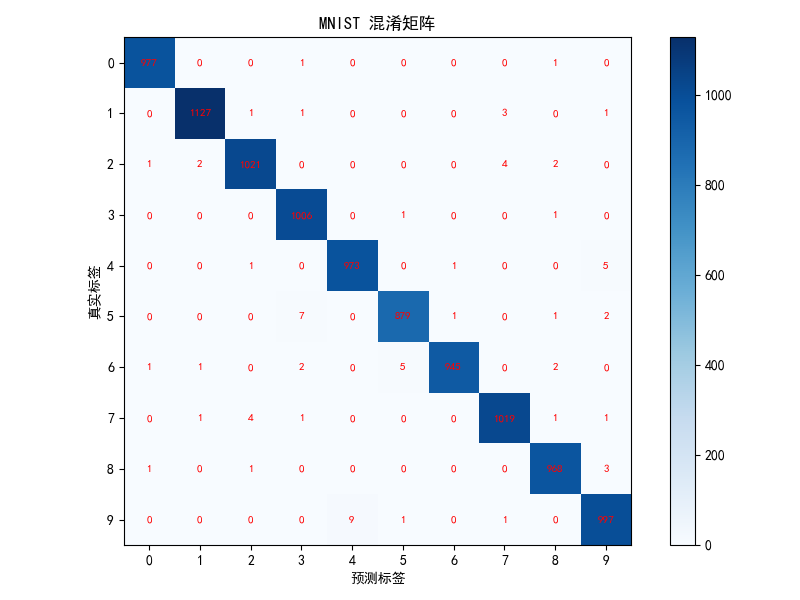
\includegraphics[width=0.6\textwidth]{Figure_1.png}
    \caption{MNIST 数据集混淆矩阵}
    \label{fig:confusion_matrix}
\end{figure}

\section{实验总结}
前馈神经网络在图像分类任务中具有良好的特征提取能力。通过本实验，加深了对神经网络结构、训练流程和模型评估方法的理解。该方法在手写识别、模式识别等实际应用中具有重要价值。


\newpage
\appendix
\section{完整代码}

\begin{lstlisting}[language=Python]
import mindspore as ms
from mindspore import nn, context, Model
from mindspore.dataset import MnistDataset
from mindspore.dataset.vision import transforms
from mindspore.dataset.transforms import Compose
import numpy as np
import matplotlib.pyplot as plt
from sklearn.metrics import confusion_matrix

plt.rcParams['font.sans-serif'] = ['SimHei']
plt.rcParams['axes.unicode_minus'] = False

context.set_context(mode=context.GRAPH_MODE, device_target="CPU")

def create_dataset(data_path, batch_size=128, repeat_size=1, shuffle=True):
    dataset = MnistDataset(data_path, shuffle=shuffle)

    image_transforms = Compose([
        transforms.Rescale(1.0 / 255.0, 0.0),
        transforms.Normalize(mean=(0.1307,), std=(0.3081,)),
        transforms.HWC2CHW()
    ])

    label_transform = transforms.TypeCast(ms.int32)

    dataset = dataset.map(image_transforms, input_columns="image")
    dataset = dataset.map(label_transform, input_columns="label")
    dataset = dataset.batch(batch_size, drop_remainder=True)
    dataset = dataset.repeat(repeat_size)
    return dataset


train_dataset = create_dataset("./MNIST_Data/train", batch_size=128)
test_dataset = create_dataset("./MNIST_Data/test", batch_size=128, shuffle=False)

class FeedForwardCNN(nn.Cell):
    def __init__(self, num_classes=10):
        super(FeedForwardCNN, self).__init__()

        self.conv1 = nn.Conv2d(1, 32, kernel_size=3, pad_mode='same')
        self.conv2 = nn.Conv2d(32, 64, kernel_size=3, pad_mode='same')
        self.conv3 = nn.Conv2d(64, 64, kernel_size=3, pad_mode='same')
        self.conv4 = nn.Conv2d(64, 128, kernel_size=3, pad_mode='same')
        self.conv5 = nn.Conv2d(128, 128, kernel_size=3, pad_mode='same')

        self.relu = nn.ReLU()
        self.pool = nn.MaxPool2d(kernel_size=2, stride=2)

        self.flatten = nn.Flatten()
        self.fc = nn.Dense(128 * 14 * 14, num_classes)

    def construct(self, x):
        x = self.relu(self.conv1(x))
        x = self.relu(self.conv2(x))
        x = self.pool(x)
        x = self.relu(self.conv3(x))
        x = self.relu(self.conv4(x))
        x = self.relu(self.conv5(x))
        x = self.flatten(x)
        x = self.fc(x)
        return x


network = FeedForwardCNN()

loss_fn = nn.CrossEntropyLoss()
optimizer = nn.Adam(network.trainable_params(), learning_rate=0.001)
metrics = {"Accuracy": nn.Accuracy()}

model = Model(network, loss_fn=loss_fn, optimizer=optimizer, metrics=metrics)

print("开始训练模型...")
model.train(epoch=5, train_dataset=train_dataset, dataset_sink_mode=False)

print("开始评估模型...")
eval_result = model.eval(test_dataset, dataset_sink_mode=False)
print("测试集准确率：", eval_result)

y_true = []
y_pred = []

for data in test_dataset.create_dict_iterator():
    images = data["image"]
    labels = data["label"]
    outputs = network(images)
    preds = outputs.argmax(axis=1)
    y_true.extend(labels.asnumpy())
    y_pred.extend(preds.asnumpy())

cm = confusion_matrix(y_true, y_pred)

plt.figure(figsize=(8, 6))
plt.imshow(cm, interpolation='nearest', cmap=plt.cm.Blues)
plt.title("MNIST 混淆矩阵")
plt.colorbar()
plt.xlabel("预测标签")
plt.ylabel("真实标签")
plt.xticks(np.arange(10))
plt.yticks(np.arange(10))

for i in range(10):
    for j in range(10):
        plt.text(j, i, cm[i, j],
                    ha="center", va="center", color="red", fontsize=8)

plt.tight_layout()
plt.show()
\end{lstlisting}

\end{document}